% !TeX root = ../main.tex

\chapter{Fundamentals} \label{chapter:fundamentals}

To get a general understanding of how training a neural network works, we have to go through its theoretical concepts first. We start with the structure of simple feed-forward networks, continue with advanced model architectures that take advantage of the data's spatial or temporal properties, and finally end up with recent enhancements that we use throughout our final implementation.


\section{Neural Networks}

The main concept of neural networks (NN) dates back to the early 1950s, Warren McCulloch and Walter Pitts tried to build a mathematical model of information processing in our brain. Inspired by this work, Frank Rosenblatt developed the so called \textit{perceptron} about two decades later \parencite[p. 226]{pattern_and_ml}. 

\subsection{Basics}

The perceptron itself is has quite a simple structure. It is usually visualized as a node that consists any number of binary inputs $ x_{i} $, as well as a single output $ y $ with $ x_{i}, y \in \{0, 1\} $. In addition, each input is weighted by $ w_{i} \in \rm I\!R $ to express importance of each particular input. The output is determined by the simple rule that the weighted sum of all inputs has to reach a specified threshold to make the perceptron fire its output \parencite{neural_nets_deep_learning}. Usually, this threshold is usually called bias $ b \in \rm I\!R $, defined as the negative threshold. All of this can be expressed as follows:

\begin{equation} \label{eq:mlp}
  y = \begin{cases}
    1, & \text{if $ \sum\limits_{i=1}^n \, w_{i}x_{i} + b > 0$},\\
    0, & \text{otherwise}.
  \end{cases}
\end{equation}

Even that its formulation is that simple, it can represent complex decision-making when we stack multiple elements togther, known as multilayer perceptrons (MLP). Such a network is illustrated in figure \ref{fig:mlp}.

\begin{figure}[htpb]
	\centering
	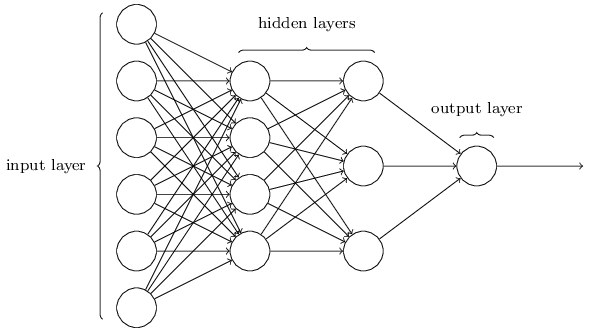
\includegraphics[scale=0.35]{figures/mlp.png} % TODO: highlight perceptron in BOLD
	\caption[Multilayer perceptron]{Example of a MLP. A single perceptron is highlighted in bold.} \label{fig:mlp}
\end{figure}

The first and last layer of such a network are refered as \textit{input layer} and \textit{output layer} and their number is determined by the given problem to solve. In case we want to train a network that identifies human faces in colored pictures with height and width of 100 pixels, it would require our input layer to have $ n_{input}=3000 $ perceptrons, as well as a single output. In contrary, all intermediate layers are known as \textit{hidden layers} and can have any number of elements and depth. When every node from one layer is connected to all nodes of its subsequent layer, we call it \textit{fully connected} (FC).

Afterwards, we can feed the input layer with a data example and apply equation \ref{eq:mlp} in each node to retrieve our binary result. This prediction step is called \textit{inference}. But in order to retrive meaningful results, we have to train our network first.

\subsection{Network Training}

The final goal of training such a network is to end up with a model that generalizes on any kind of data from the same class \parencite[p. 2]{pattern_and_ml}. The data that is used during this process is called \textit{training set}, the data that evaluates its generalization capabilites \textit{test set}. Since we know the ground truth outcome of this data example during the training phase, we can quantify the outcome using a loss function\footnote{Also known as cost function, objective function or error function. We use the averaged variants for all presented functions, because therefore we achieve pixel-wise results that are independent regarding the image dimensions later on when performing frame prediction. Additionally, the non-averaged versions of MAE and MSE are known as $ \ell_{1} $ and $ \ell_{2} $.}, such as \textit{mean absolute error} (MAE):

\begin{equation} \label{eq:mae}
  \mathcal{L}_{MAE}(w, b)=\frac{1}{N} \sum\limits_{x} | y(x) - t(x) |
\end{equation}

\textit{mean squared error} (MSE):

\begin{equation} \label{eq:mse}
  \mathcal{L}_{MSE}(w, b)=\frac{1}{N} \sum\limits_{x} \| y(x) - t(x) \|^2
\end{equation}

or \textit{binary cross-entropy} (BCE) \parencite{conv_lstm_nowcasting}:

\begin{equation} \label{eq:bce}
  \mathcal{L}_{BCE}(w, b)= -\frac{1}{N} \sum\limits_{x} t(x) \log{(y(x))} + (1-t(x)) \log{(1-y(x))} 
\end{equation}

where $ N $ is the number of examples and $ t(x) $ denotes the ground truth target of an input example $x$. Many other functions exist, but these are the main objectives that we use in later chapters. During training our network, we want to find the set of weights $ w $ and biases $ b $ that minimizes our error:

\begin{equation} \label{eq:min-loss}
  arg\min_{w, b} \mathcal{L}(w, b)
\end{equation}

Parameters beside $ w $ and $ b $ that are not learned during this process are called \textit{hyperparameters}. An example of such an non-trainable parameters are the number of layers or the size of each single layer. More hyperparameters will arise in the next sections.


\subsubsection{Neurons and Activations}

At this point, we face the fundamental problem of perceptrons. Because in order find the best set of parameters, we have to do small changes in $ w $ and $ b $ to justify the output into the right direction of the desired outcome. But since the perceptron's output is discrete, a small change can cause a sudden flip in the overall output. To overcome this issue, we replace these perceptrons with \textit{neurons}:

\begin{equation}
\begin{aligned}
z &= \sum\limits_{i=1}^n \, w_{i}x_{i} + b \\
y &= a(z)
\end{aligned}
\end{equation}

which allow $ x_{i}, y \in \rm I\!R $ by wrapping its term with a non-linear \textit{activation function} $ a(z) $. Frequently used examples are the sigmoid function $ \sigma(z) $, hyperbolic tangent $ tanh(z) $ and the rectified linear unit (ReLu) $ max(0, z) $. These are displayed in figure \ref{fig:activations}.

\begin{figure}[htpb]
  \centering
  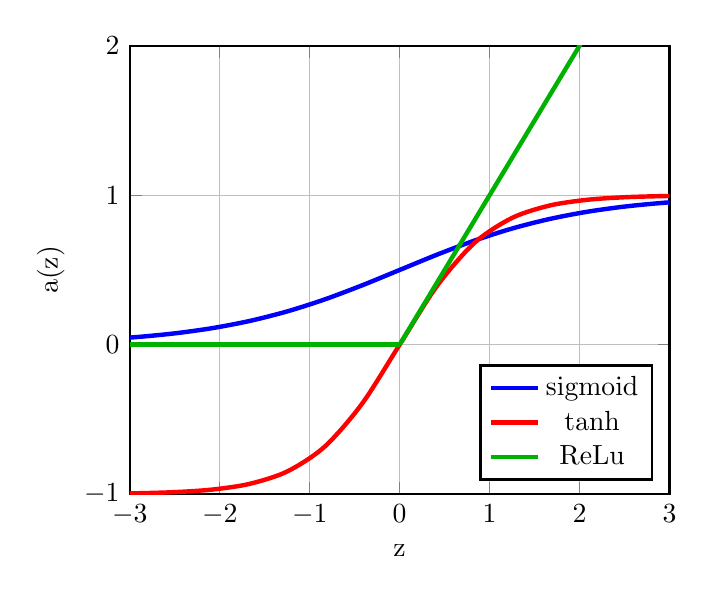
\begin{tikzpicture}
    \begin{axis}[
        ymin=-1,
        ymax=2,
        xmin=-3,
        xmax=3,
        legend style={legend pos=south east},
        grid,
        thick,
        ylabel=a(z),
        xlabel=z
      ]
      \addplot [mark=none,draw=blue,smooth,ultra  thick] {1/(1+exp(-1*(\x))};
      \addlegendentry{sigmoid};
      \addplot [mark=none,draw=red,smooth,ultra thick] {tanh(\x)};
      \addlegendentry{tanh};
      \addplot[mark=none,draw=black!30!green,ultra thick,smooth,domain=0:3] {x};
	  \addplot[mark=none,draw=black!30!green,ultra thick,smooth,domain=-3:0] {0};
      \addlegendentry{ReLu};
    \end{axis}
  \end{tikzpicture}
  \caption[Activation functions]{Diagram showing the most common activation functions in neural networks.}\label{fig:activations}
\end{figure}

Note that the sigmoid function's shape is a smoothed out variant of the \textit{step function} \parencite{neural_nets_deep_learning}, which can be used to make a neuron act like a perceptron. Additionally, the rectifier differs to both other activation functions in that it is one-sided and partly linear. Even its shape looks much simpler, it became the most favorable activation function for intermediate layers in deep neural networks, as it allows faster computation, sparse activation\footnote{{A sparse activation means that only half of the neurons will have an initial non-zero output, when a uniform initialization is used.}}, reduces the likelihood of vanising gradient (see \ref{sec:rnn-drawbacks}) and is more biologically plausible \parencite{relu}.

\subsubsection{Initialization}

Before starting the training process, we have to assign each variables $ w $ and $ b $ an initial value. This is done by pure randomness, using for example a uniform or gaussian distribution. But if we start with weights that are too small, the signal can decrease so much that it is to small to be usefull. On the other side, when we initialize our parameters with high values, the signal can end up to explode while propagating through the network \parencite{understand_xavier}. In consequence, a good initialization has a radical effect on how fast the network will learn useful patterns.

For this purpose, some best practices have been developed. One famous example that is used throughout in our final model is \textit{Xavier initialization} (eq. \ref{eq:xavier}). Its formulation is based on the number of input and output neurons and uses sampling from an uniform distribution with zero mean and all biases set to zero \parencite{xavier-init}:

\begin{equation} \label{eq:xavier}
  W \sim \mathcal{U} \bigg[-\sqrt{\frac{6}{n_{in} + n_{out}}}, \sqrt{\frac{6}{n_{in} + n_{out}}}\bigg]
\end{equation}

where $ W $ is the weight matrix at each layer, $ n_{in} $ the number of incoming connections and $ n_{out} $ the number of outgoing connectons to the next layer. This initialization is designed to keep the gradients in all layers within approcimately the same scale.

\subsubsection{Backpropagation Learning Algorithm}

To acually train the network by minimizing its error (eq. \ref{eq:min-loss}), we apply a learning alogrithm called \textit{backpropagation}. This algorithm is based on \textit{gradient descent}, which iteratively tries to find the minima of a function by doing small steps towards the negative gradient. Applying this to our loss function results in the \textit{update rule} for all weights and biases:

\begin{equation} \label{eq:gradient_descent}
\begin{aligned}
w_{i}^{(\tau + 1)} &= w_{i}^{(\tau)} - \eta \frac{\partial \mathcal{L}}{\partial w_{i}^{(\tau)}} \\
b_{j}^{(\tau + 1)} &= b_{j}^{(\tau)} - \eta \frac{\partial \mathcal{L}}{\partial b_{j}^{(\tau)}}
\end{aligned}
\end{equation}

where $ \eta > 0 $ is the \textit{learning rate} that determines the size of step we do along the slope in each iteration \parencite{pattern_and_ml}. Doing such a single step by computing the gradients for the whole training set would require to much time and memory resources. Hence, we estimate the gradients over the whole population by using a smaller sample. This technique is called \textit{stochastic gradient descent} (SGD), whereas the size of the sample is known as \textit{batch size}.

Although this algorithm is really powerful, it comes with some disadvantages that have to be kept in mind. First, the result can converge to any local minimum. In consequence, finding a global minimum is not guaranteed. Secondly, depending on the choice of the learning rate $ \eta $, the algorithm might converge very slowly or even not at all \parencite{ann}.

Beside SGD, many other advanced gradient descent based optimization algorithms exist. Detailed explainations and visualizations can be found in \parencite{optimization}. The optimizer that is used in this thesis is called \textit{adaptive moments estimation} (Adam). This algorithm is based on adaptive estimates of lower-order moments and performs a form of step size annealing by using exponential moving averages of the parameters. Therefore, it usually requries less tuning of the learning rate and has shown to work well in practice \parencite{adam}.


\subsubsection{Stopping Criteria}

The training process can run endless. Therefore, a rule should be defined when to stop it. There are many options when to cancel the training. Also, combinations of different stopping criterias are possible. These can be for example:

\begin{itemize}
\item When the validation loss does not decrease (for a specified number of iterations).
\item When the change in loss falls below a defined threshold (for a specified number of iterations).
\item When a fixed number of steps or epochs\footnote{A single epoch is usually defined as the number of steps that is required to iterate over the whole trainng set.} elapses.
\item When a defined timeframe exceeds.
\end{itemize}


\subsection{Regularization}

As already stated, our goal is to find a representation that generalizes well. One common problem that has to be prevented when a neural network is trained is the effect of \textit{overfitting}. This means that even the training loss decreases further and further, the validation and test error suddenly starts to get worse. One cause might be that the size of the training set is not large enough. But to come up with more data is often not possible. Another reason might be that our \textit{model complexity}, so the total number of trainable parameters to high. To get an idea about the reason for this, imagine we want to fit a function $g(x)$ using some noisy data points of a ground truth function $f(x)$. When our model exhibits to many parameters, it might come up with a function that fits perfectly to all data points. Nevertheless, as demonstrated in figure \ref{fig:overfitting}, this is a bad regression of the unterlying function $f(x)$.

\begin{figure}[htpb]
  \centering
  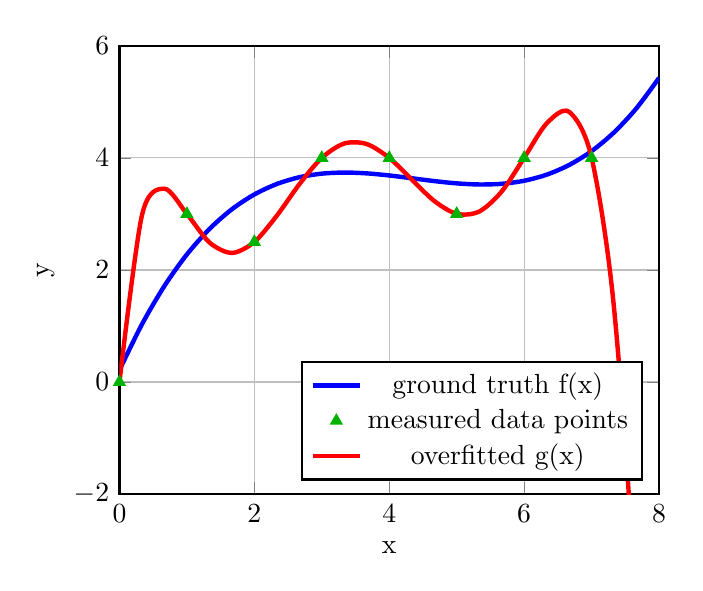
\begin{tikzpicture}
    \begin{axis}[
        ymin=-2,
        ymax=6,
        xmin=0,
        xmax=8,
        legend style={legend pos=south east},
        grid,
        thick,
        ylabel=y,
        xlabel=x,
        scatter/classes={%
		a={mark=triangle*,black!30!green}}
      ]
      \addplot [mark=none,draw=blue,smooth,ultra thick, domain=0:8] {
		 0.21212121212121271*x^0
   		+2.6607142857142843*x^1
  		-0.64502164502164450*x^2
   		+0.049242424242424192*x^3  
      };
      \addlegendentry{ground truth f(x)};
      \addplot[scatter,only marks,%
		scatter src=explicit symbolic]%
	table[meta=label] {
	x     y      label
	0     0      a 
	1     3      a
	2     2.5    a 
	3     4      a 
	4     4      a 
	5     3      a 
	6     4      a 
	7     4      a 
	};
	\addlegendentry{measured data points};
	\addplot [mark=none,draw=red,smooth,ultra thick, domain=0:8] {
		-0.0000000003717474*x^0
   		+14.921428855475133*x^1
  		-22.184722849828937*x^2
   		+13.906250509793455*x^3
  		-4.2638890895127091*x^4
   		+0.67083337448114122*x^5
  		-0.051388893117505295*x^6
   		+0.0014880954099440117*x^7
      };
      \addlegendentry{overfitted g(x)};
    \end{axis}
  \end{tikzpicture}
  \caption[Regularization and overfitting]{Visualization of an overfitted function.}\label{fig:overfitting}
\end{figure}

On the other hand, a reduction of model complexity can also be a false conclusion because this limits the potential power of the network as well. Fortunately, research has originated different methods to master this issue.

A well known technique to delimitate overfitting is to penetalize high parameter values which cause the oscillation effect that can be seen in figure \ref{fig:overfitting}. Therefore, we extend our loss function with an additional regularization term. This method is called weight decay:

\begin{equation} \label{eq:reg-loss}
  \mathcal{L}_{total}(w, b)= \mathcal{L}(w, b) + \frac{\lambda}{N} \sum\limits_{w}w^2
\end{equation}

where the coefficient $ \lambda $ controls the influence of the regularization. The example shown in eq. \ref{eq:reg-loss} uses an $ \ell_{2} $ regularizer over all weigths, which strongly penetalizes a high magnitude of values. Together with the learning rate $ \eta $, both define two of the most important hyperparameters in any neural network model. Finding appropriate values is a major task when finetuning the model.

A second regularization approach is known as \textit{dropout}. Instead of modifying the cost function, it manimulates a model's layer where it is applied on by randomly deactivating a neuron with a probability $p$ in every training step. As a result, the networks learns a robustness against distint patterns that cause a high activation towards a certain output. Stated differently, the network is forced not to learn any shortcut that could damage generality. It is to add that no neuron is deactivated during inference. But to compensate the higher amout of active neurons within the layer, all weights of outgoing connections will be multiplied by $ p $ \parencite[p. 1931]{dropout}



\section{Convolutional Neural Networks}

In the previous section, we have discovered neural networks that exhibits a full connection of neuros from one layer to the next. While this allows to learn complex representions on the one hand, it comes with a couple of downside on the other hand as well. For example, data such as images would require the nework's layers to become large. Consequently, the number of connections between these layers would increase exponentially and thus the amound of trainable parameters as well. At the bottom line, this could end up in a network that is either time-consuming to train, or we are even not able to store it in memory. In addition, we would not not take any advantage of local image properties into account.

Therefore, a new network type found attention in recent years that are known as \textit{convolutional neural networks} (CNN). It is inspired by the animals visual cortex, has already been used in the late nineties to solve optical character recognition tasks (OCR) \parencite{lecun_conv}, but received its main attention after beating proven methods in the ImageNet competition by a large margin \parencite{imagenet}. The structure of a convolutional network, the detailed benefits and its mathematical formulation is described in the following sections.


\subsection{Structure}

A network is called CNN, when it consists of at least one convolutional layer. In other words, ``\textit{convolutional networks are simply neural networks that use convolution in place of general matrix multiplication in at least one of their layers.}'' \parencite{deep_learning}. The definition of the convolution operation follows in section \ref{sec:conv-op}. Simply put, imagine a small window that slides across the input data. In every iteration, it attempts to extract features that are only dependent on a small neighbouring region with the size of this window. Moreover, the location of features that it tries to detect is not fixed to any specific spot, as it treats every patch in the same way. In every convolutional layer, this process is repeated several times, resulting in multiple feature maps. Figure \ref{fig:cnn-structure} visualizes the described structure of a simplified convolutional neural network.

\begin{figure}[htpb]
	\centering
	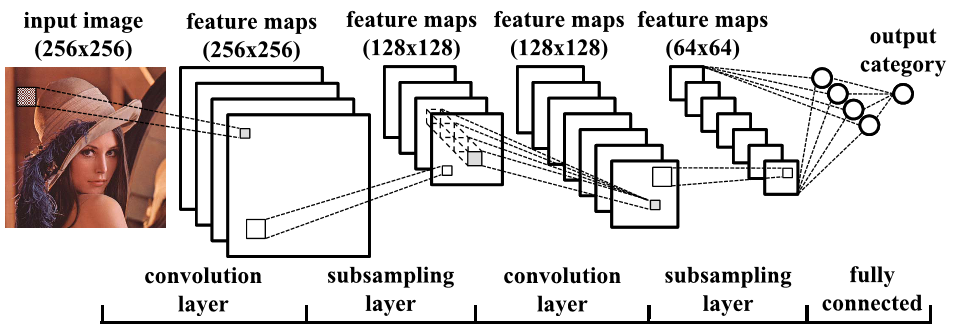
\includegraphics[scale=0.35]{figures/cnn_structure.png}
	\caption[Structure of a CNN]{Example of a simplified CNN structure with two convolutional layers for image classification.} \label{fig:cnn-structure}
\end{figure}

The window mentioned before is called \textit{kernel} and holds the randomly initialized parameters that the network can learn. The kernel acts as a filter that is applied to each location in a regular steps. In the two dimensional case, the kernal has a specified width and height, denoted as \textit{kernel size}. Several kernals are used to extract multiple feature maps in each convolutional layer, but each output feature map is computed with its own kernel. This number of kernels is specified with its \textit{kernel depth}. Furthermore, the step range the filter is moved in each dimension is called \textit{stride} \parencite{conv_guide}.

Each convolutioal layers is usually followed by a non-liner acitivation function, preferably a rectifier. The reason is that the convolution is an affine transformation and it therefore linear. Stacking multiple linear operations could be mathematically reduced to as single one. Optionally, an additional \textit{pooling layer} can be applied that performs a subsampling onto the feature maps. Several pooling variants exist, while \textit{max pooling} is probably the most frequently used of them. It allows the representation to become roughly invariant to small rotations or translations of the input \parencite[p. 343]{deep_learning} by only using the maximum value.


\subsection{Convolutional Operation} \label{sec:conv-op}

Generally speaking, the convolution in an mathematical operation on two functions $f(x)$ and $g(x)$. Its operator is typically denoted with an asterisk \parencite[p. 332]{deep_learning} and is defined as:

\begin{equation} \label{eq:conv-general}
  (f \ast g)(x) = \int f(\tau)g(x-\tau) d\tau
\end{equation}

In terminology of convolutional networks, the function $f$ is termed as the \textit{input} and the filter $g$ is referred to as the \textit{kernel}. Moreover, the output of $ (f \ast g)(x) $ is called the \textit{feature map}.

As we are dealing with discrete 2D-images in this thesis, the formulation of equation \ref{eq:conv-general} can be discritized and reformulated as:

\begin{equation} \label{eq:conv-2d}
  (I \ast K)(x,y) = \sum\limits_{r=0}^{h-1} \sum\limits_{c=0}^{w-1} I(c,r)K(x-c,y-r)
\end{equation}

with an input $ I $ of size $w \times h$ and a two-dimensional kernel $ K $. Depending on the size of the kernel with $ k \times k $ and the chosen stride $ s $, the shape of the convolved output changes. This is why in input is often enriched with a \textit{zero-padding} to have more control regarding the resulting output size. The use of no padding ($p=0$) is also called \textit{valid padding} (Figure \ref{fig:conv_valid}). Also, when a padding of $p=\floor{k/2}$ is used with a kernal size, it is referred to as \textit{same padding} because the input and output size stay unchanged in case of $ s=1 $ (Figure \ref{fig:conv_same}). 

\begin{figure}[htpb]
\centering
\begin{subfigure}{0.5\textwidth}
  \centering
  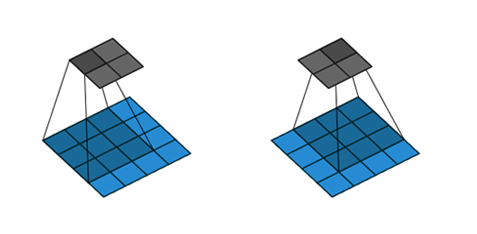
\includegraphics[width=.9\linewidth]{figures/conv_valid.png}
  \caption{$p=0$ (valid), $s=1$}
  \label{fig:conv_valid}
\end{subfigure}%
\begin{subfigure}{0.5\textwidth}
  \centering
  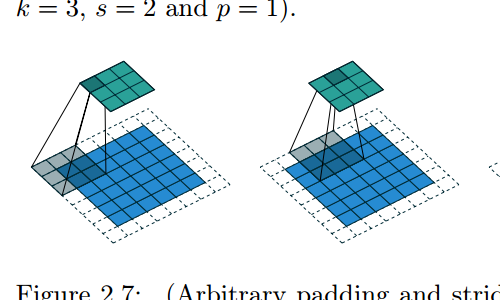
\includegraphics[width=0.9\linewidth]{figures/conv_same.png}
  \caption{$p=1$ (same), $s=2$}
  \label{fig:conv_same}
\end{subfigure}
\caption[Convolution operation]{Visualizations of the convolutional operation with an $3 \times 3$ kernel but different settings for padding and stride.}
\label{fig:conv}
\end{figure}

It must be noted that the size of the kernel, padding and stride does not have to be equal in each dimension. But nevertheless, this is the case in most practical applications.

\subsection{Transposed Convolutional Operation}

The application of the previously presented convolutional operation usually transforms the input into lower-dimensional feature maps. However, there are use cases where we would like to go the other way round, while keeping the connectivity pattern of a convolution. One example is an convolutional autoencoder which is explained in further detail in section \ref{sec:autoencoder}. This operation is referred to as \textit{transposed convolution}\footnote{Mistakenly, the transposed convolution is often called \textit{deconvolution}. But because it is not actually performing the reverse effect of a convolution, which is meant by the mathematical term of a deconvolution, it is strongly discouraged to name it so.}, which exchanges the forward and backward passes of a normal convolution. It is also called \textit{fractionally strided convolution}, because it can be emulated with a direct convolution using a zero-spaced input \cite[p. 19]{conv_guide}. Such an implementation is less efficient, but it supports the intuition of how the resulting output shape looks like. Figure \ref{fig:conv_tp} shows an example of a transposed convolution.

\begin{figure}[htpb]
	\centering
	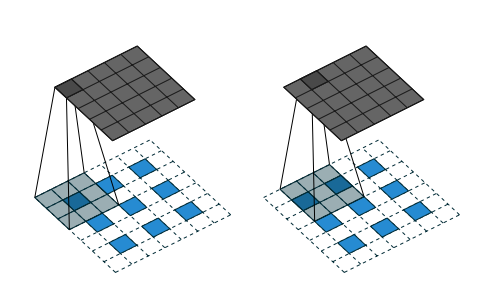
\includegraphics[scale=0.4]{figures/conv_tp.png}
	\caption[Transposed convolution operation]{Transposition of convolving an $6 \times 6$ input using a $3 \times 3$ kernel using $p=1$ and $s=2$. This is equivalent to performing an convolution using zero-space $3 \times 3$ input with $p=1$ and $s=1$.} \label{fig:conv_tp}
\end{figure}


\subsection{Advantages}

To sum up the benefits of an convolutional network, the three central design ideas are \textit{sparse connections}, \textit{parameter sharing} and \textit{equivariance to translation} \parencite[p. 336ff.]{deep_learning}.

\begin{figure}[htpb]
\centering
\begin{subfigure}{0.5\textwidth}
  \centering
  
\includegraphics[width=.9\linewidth]{figures/placeholder.png}
  \caption{}
  \label{fig:conv_vs_fc_fc}
\end{subfigure}%
\begin{subfigure}{0.5\textwidth}
  \centering
  
\includegraphics[width=0.9\linewidth]{figures/placeholder.png}
  \caption{}
  \label{fig:conv_vs_fc_conv}
\end{subfigure}
\caption[Sparse connections and parameter sharing in a CNN]{Comparison of the connection pattern and usage of parameters between (a) fully-connected layers and (b) convolutional layers.}
\label{fig:conv_vs_fc}
\end{figure}

\subsubsection*{Sparse Connections}

The kernel used in a convolution is smaller than in input. Consequently, we have to store fewer parameters, as well as can take advantage of local relationships present in the data. This also leads to a higher training efficiency and a radical reduction of memory requirements.

\subsubsection*{Parameter Sharing}

To handle all regions of the input data in the same manner, the parameters are reused at every location as well. This is implemented by making use of only a single kernel which holds all learnable parameters.  Additionally, this decreases the number of parameters even further. To that end, figure \ref{fig:conv_vs_fc} compares the connection pattern  and the sharing of model parameters of fully-connected layers against the convolutional case.

\subsubsection*{Equivariance to Translation}

The sharing of parameters leads to the third advantage. Because the kernel and its paramters are reused at every position, the model learns the same representations at every position \parencite[p. 339]{deep_learning}. For example, if an input image wis translated by a fixed number of pixels, the network would handle it in the same way.

Unfortunately, convolutions are not tolerant to other transformations like rotation from the ground up. But to counteract this, other techniques exist such as a subsequent pooling stage as already introduced before.


\subsection{Fully-Convolutional Networks}

The complete use of convolutional layers implicates a fourth advantage over fully-connected layers. Since the kernel size in each layer is independent regarding its input, the overall network could be feed with data of different dimension. In contrary, this is not possible anymore as soon as a single FC-layer is used at inference because its fixed-sized weight matrix has to be applied to the entire input, not just a local region. Nevertheless, this does not imply that no fully-connected layer can be used when training the network. Depending on the architecture, FC-layers can be used in components of the network that are only used during training. This advantage is for example taken into account when training a \textit{deep convolutional generative adversarial network} (DCGAN)\footnote{Novel network training strategy for generative networks, where a generator network G competes agains a second discriminator network D in an alternating fashion. Further details in \parencite{gan}.}, whose discriminator network is only used while training.

Regarding the problem of frame prediction we want to solve within this thesis, we have to deal with a huge amount of data in every training iteration. Therefore, we take advantage from this \textit{fully-convolutional network} (FCN) approach and design our architecture in such a way that we are able train neural network model on small image patches only. Afterwards, we can theoratically perform frame prediction on the whole image given a sequence of frames.


\section{Recurrent Neural Networks}

Networks for temporal learning...

\subsection{RNN}

Bla bla...

\subsubsection{History}
Short intro (history) to RNNs

\subsubsection{Architecture}
explain it in with a small diagram

\subsubsection{BPTT}
What is BPTT in comparision to back propagation

\subsubsection{Drawbacks} \label{sec:rnn-drawbacks}
What are the drawbacks of RNNs: vanishing/explosion of gradients problem

\subsection{LSTM}

Bla bla

\subsubsection{History}
Short intro (history) to LSTMs (Hochreiter, Schmidhuber)

\subsubsection{Architecture}
Show differences to classical RNNs

\subsubsection{Benefits}
How does this suspensate the drawbacks of RNNs (gates, ...)


\section{Autoencoder Networks} \label{sec:autoencoder}

What are autoencoder networks?


\section{Batch Normalization}


\section{Perceptuall Similarity of Images}

Introduce perceptual similarity and explain some metrics (SSIM, PSNR, GDL?) which we will use in evaluation.
Why is perceptuall loss so important? Example of chess/zebra image?

